\section{Initialization}

\subsection{Manual}
As suggested in the project statement, manual initialization
was implemented first to evaluate the fitting algorithm and
the automatic initialization separately.

The implementation is pretty straightforward. Using different
OpenCV routines, the mean shape can be dragged to its initial
position, and one it has been located, the fitting algorithm starts.

Nevertheless, this procedure presents a problem. The rotation of the
shape can't be changed, which causes that the initial estimation is not
as accurate as it could be.

\subsection{Automatic}

What really would make a difference in object detection is to make it automatic,
and not having to drag a shape, for each object to be detected, in each image.
Our first approach to make an automatic model was using histogram of oriented
gradients (HOG), combined with training a support vector machine (SVM), to
detect the shape of the 8 incisives altogether. But we stumbled upon an
obstacle. Whereas with other images (much more clear, less noise, with highly
detailed edges) this method is feasible, with our images it was not as good,
even after treating the image with techniques (such as denoising, white and
black hat...) The following images represent an example with a normal image, 
and one cropped section of incisives, from radiograph1.

\begin{figure}[h]
  \centering
  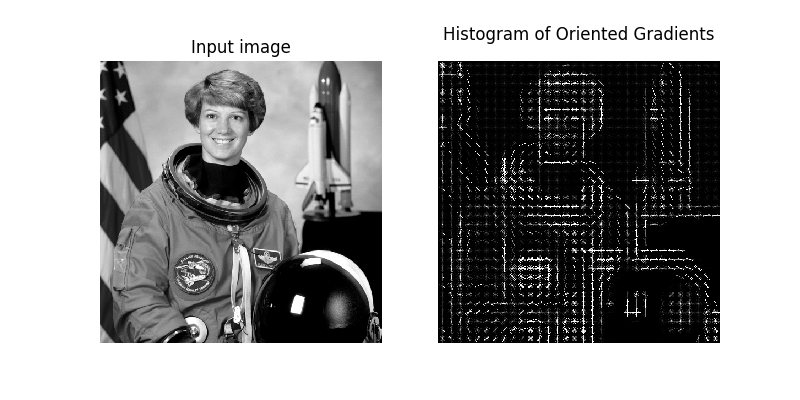
\includegraphics[height=6cm]{img/astro_hog}
  \caption{Normal image and its HOG}
\end{figure}

\begin{figure}[h]
  \centering
  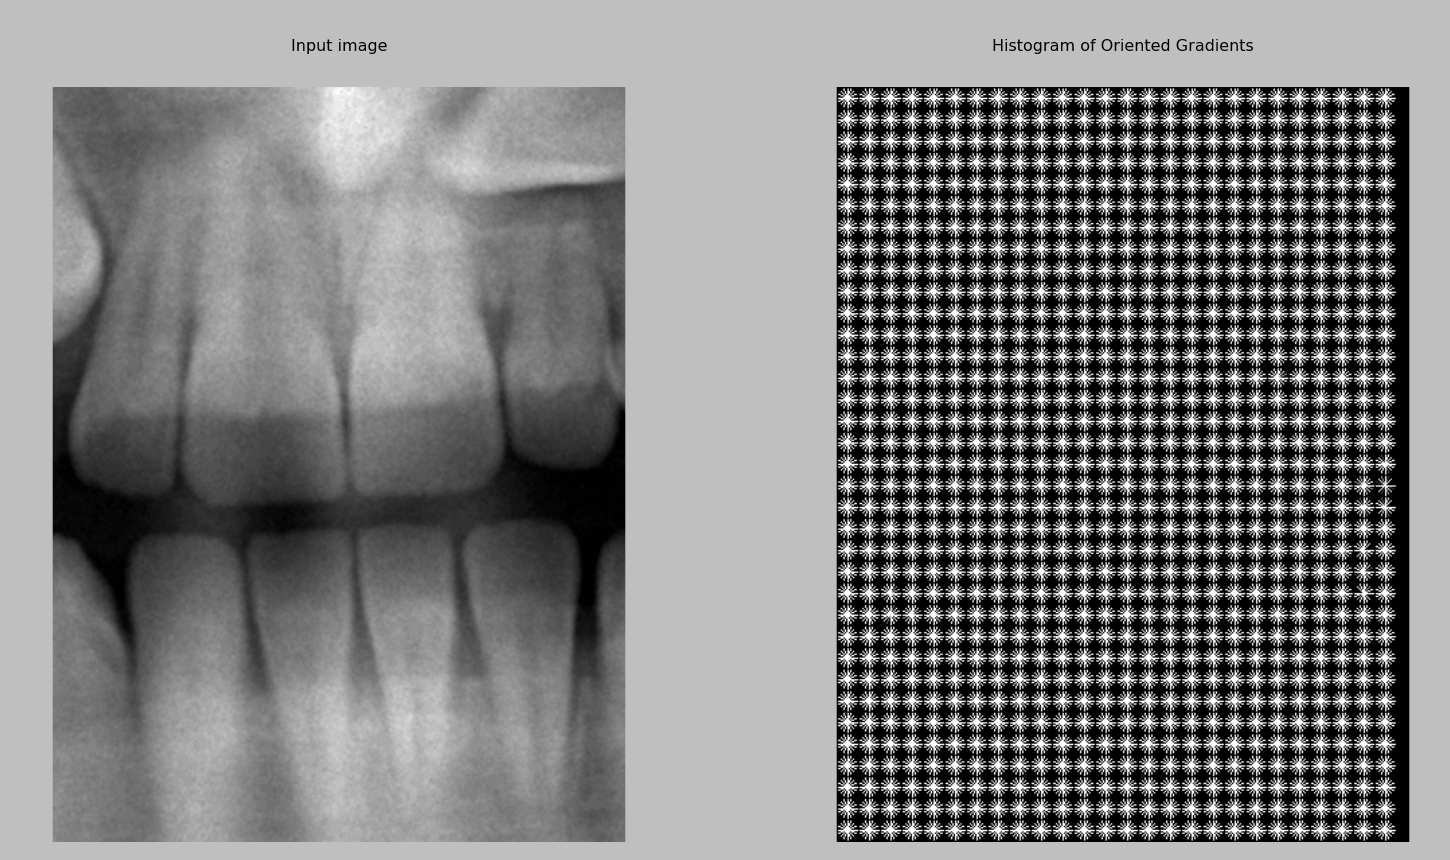
\includegraphics[height=5cm]{img/teeth_hog}
  \caption{Cropped teeth section}
\end{figure}

After that, we opted for using the Viola-Jones detection technique. With this
technique, some "basic" features are used to train a cascade classifier, which
consist of several "weak" classifiers, boosted by the appending of one afther
the other. The results obtained are good enough, but not better. The gist of
the Viola-Jones technique is that it is quite fast, but it is not flawless, and
it found quite some false positives, as shown in the image below

\begin{figure}[h]
  \centering
  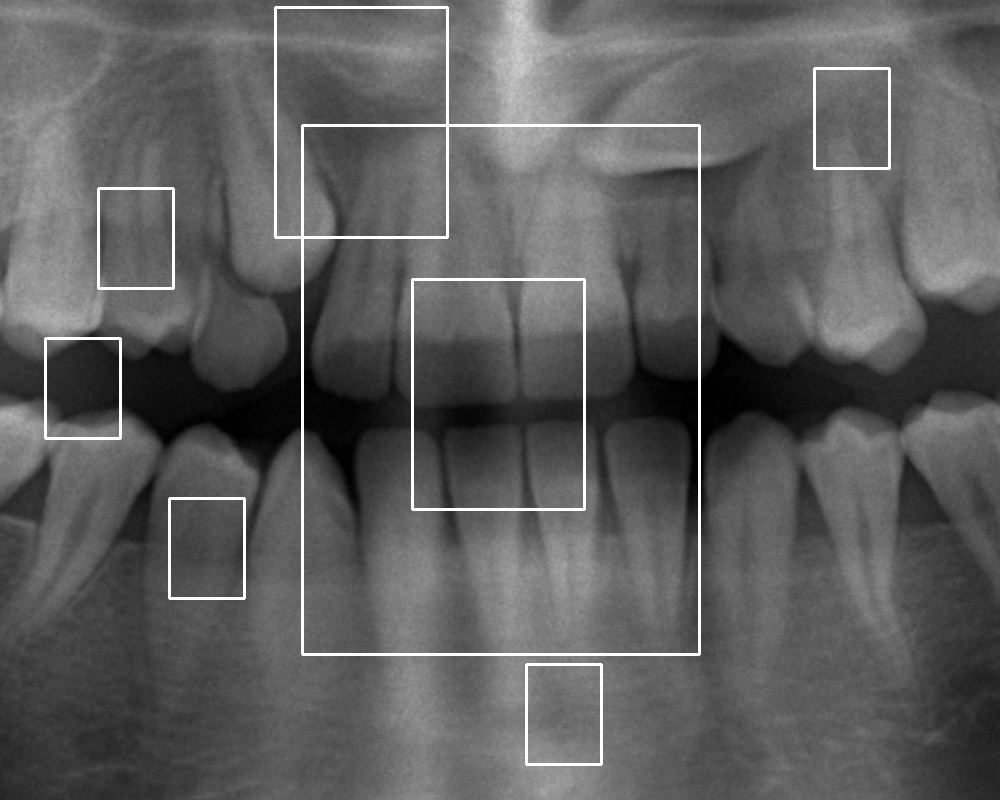
\includegraphics[height=6cm]{img/teeth_detection_1}
  \caption{Initial results of Viola-Janes detection}
\end{figure}

As can be seen, there is one very good match, and several bad matches. For this
matter, what we did in order to correct the results is, first delete rectangles
that are inside of others, and then proceed to ignore those that are not
sufficiently large enough. With these two techniques, we have a result such as
this

\begin{figure}[h]
  \centering
  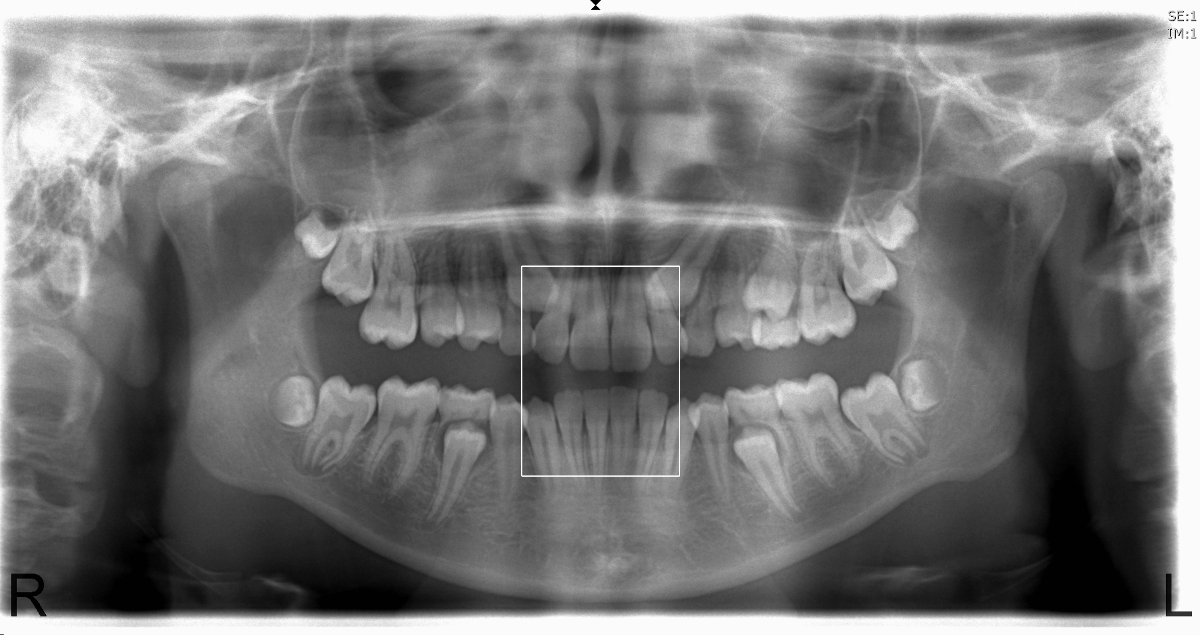
\includegraphics[height=6cm]{img/teeth_detection_2}
  \caption{Improved results}
\end{figure}

